\documentclass[seagull]{beamer}
\usetheme{AnnArbor}
\usepackage[utf8]{inputenc}
\usepackage{amsmath}
\usepackage{amsfonts}
\usepackage{amssymb}
\usepackage{graphicx}
\usepackage{minted}
\usepackage{tikz}
\usetikzlibrary{mindmap,trees}
\usepackage{verbatim}
\author{Jorge A. Medina Oliva - Barcelona/Spain}
\title{SQLAlchemy "the" python ORM}
%\setbeamercovered{transparent} 
%\setbeamertemplate{navigation symbols}{} 
\logo{} 
%\institute{} 
%\date{} 
\date{May. 22 , 2014}
%\subject{} 
\begin{document}

\begin{frame}
\titlepage
\end{frame}

%\begin{frame}
%\tableofcontents
%\end{frame}

\begin{frame}{What is an ORM?}

An ORM is the data abstraction layer in a object oriented world 
who maps tables in a relational database with object to the business logic

\end{frame}

\begin{frame}{Like what?}
\begin{itemize}
	\item Java = Hiberante
	\item PHP = Doctrine
	\item ruby = DataMapper
	\item .Net = NHibernate
\end{itemize}
\end{frame}

\begin{frame}{Like What?}
\begin{itemize}
	\item What happen in python about django?
the best known is django ORM but require django framework to work outside django
but wait exist SQLAlchemy the best ORM in the python world ( is the only one )

Let me introduce you to SQLAlchemy

The most important think is the documentation
Good documentation very helpful at http://www.sqlalchemy.org
I use it with python 2.4 to  3.3 without problems
SQLAlchemy evolve really good and is heavy used in Openstack, reddit, mozilla and other organizations
\end{itemize}
\end{frame}

\begin{frame}
\centering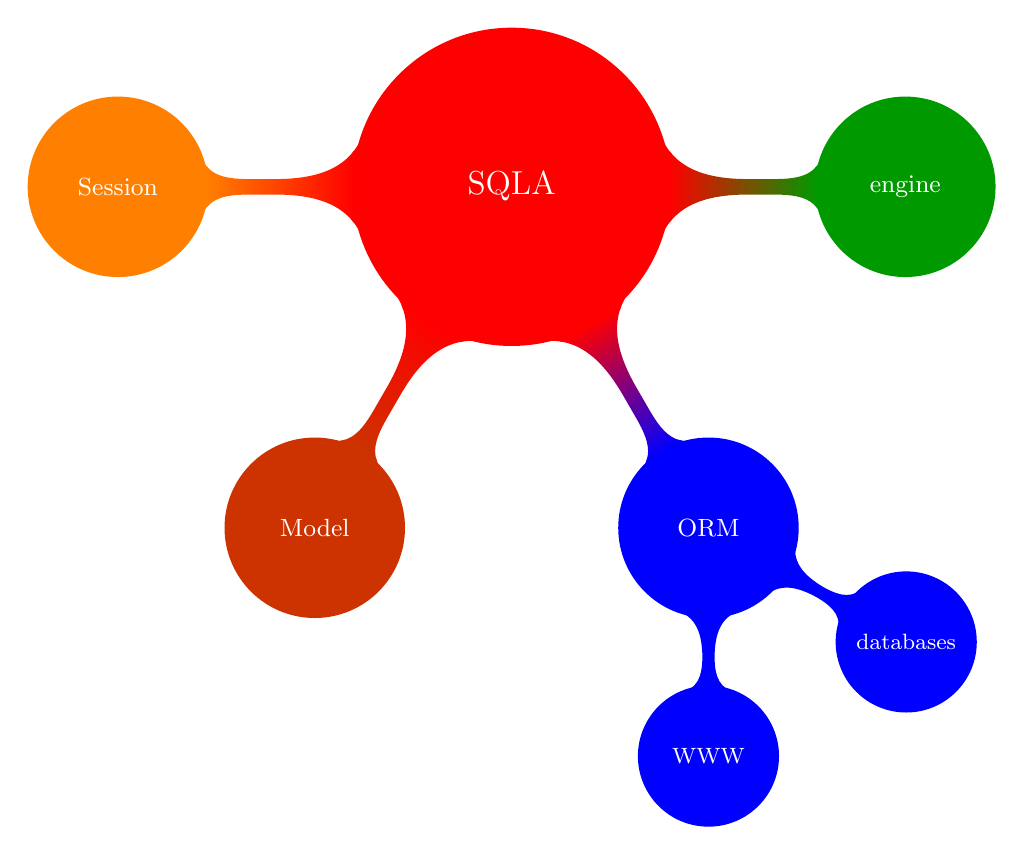
\begin{tikzpicture}
  \path[mindmap,concept color=red,text=white]
    node[concept] {SQLA} [clockwise from=0]
    child[concept color=green!60!black] {node[concept] {engine}}  
    child[concept color=blue] {
    	node[concept] {ORM}[clockwise from=-30]
      	child { node[concept] {databases} }
      	child { node[concept] {WWW} }
    }
    child[concept color=red!80!green] { node[concept] {Model} }
    child[concept color=orange] { node[concept] {Session} };
\end{tikzpicture}
\end{frame}

\begin{frame}
    \frametitle{Python and Py-Ramesses}
    \inputminted{python}{filename.py}
\end{frame}
%end presentation
\end{document}